\section{Software description}
\label{section:software}

\subsection{Software components}

\subsubsection{preCICE}

preCICE \cite{Chourdakis:2022} is an open-source coupling library for partitioned multi-physics simulations. An overview of its concept is shown in Figure \ref{fig:precice:overview}. In preCICE terminology, the coupled simulation programs are called \textit{solvers} or \textit{participants}. preCICE connects different solvers to perform a partitioned simulation. It takes care of different coupling aspects such as data mapping and communication. Different coupling schemes are possible \cite{Gatzhammer:2014} by the choice of which solvers are coupled, what data is exchanged and which coupling algorithms are used. Explicit and implicit coupling schemes are available, as well as the option to connect more than two participants via multi-coupling. In addition, preCICE provides acceleration algorithms to reach a decent computation time for large simulations and time interpolation for the coupling of solvers with different time steps. The coupling scheme is defined in the \textit{precice-config.xml}, the only global file which is accessed by all participants.\\
For each solver, a specific \textit{adapter} is necessary to communicate with preCICE. The adapter is an additional software layer which can take many forms, depending on the solver. For example, the OpenFOAM adapter is a C++ function object, an independent library, while the FEniCS adapter is a Python module. Additional language bindings in Fortran, Julia and Matlab allow the development of adapters in these languages as well.

Additional remarks: library approach, scalability, HPC

\begin{comment}

\begin{itemize}
	\item An overview is shown in Figure \ref{fig:precice:overview}
	\item Coupled simulation programs are called \textit{solvers} or \textit{participants}
	\item preCICE connects different solvers to perform a partitioned simulation
	\item preCICE takes care of different coupling aspects such as data mapping and communication
	\item Different coupling schemes can be implemented: Who is coupled o whom, what data is exchanged, which coupling algorithms are used \cite{Gatzhammer:2014}
	\item Multi-coupling: Couple multiple (in theory: arbitrary many) participants in different configurations (explicit, implicit)
	\item Acceleration: Use acceleration algorithms to reach a decent computation time
	\item Time interpolation: Use solvers with different time step sizes
	\item Coupling scheme is defined in the precice-config.xml, the only global file which is accessed by all participants
	\item For each solver, a specific \textit{adapter} is necessary to communicate to preCICE
	\item Adapter is an additional piece of software
	\item Adapter can take many forms depending on the solver, eg.: OpenFOAM - C++ Function object, FEniCS - Python module
	\item Different Language bindings are available: C/C++, Python, Fortran, Julia, Matlab
	\item The Adapter allows the solver to access preCICE and to call the coupling
\end{itemize}

\end{comment}

\begin{figure*}[h]
	\centering
	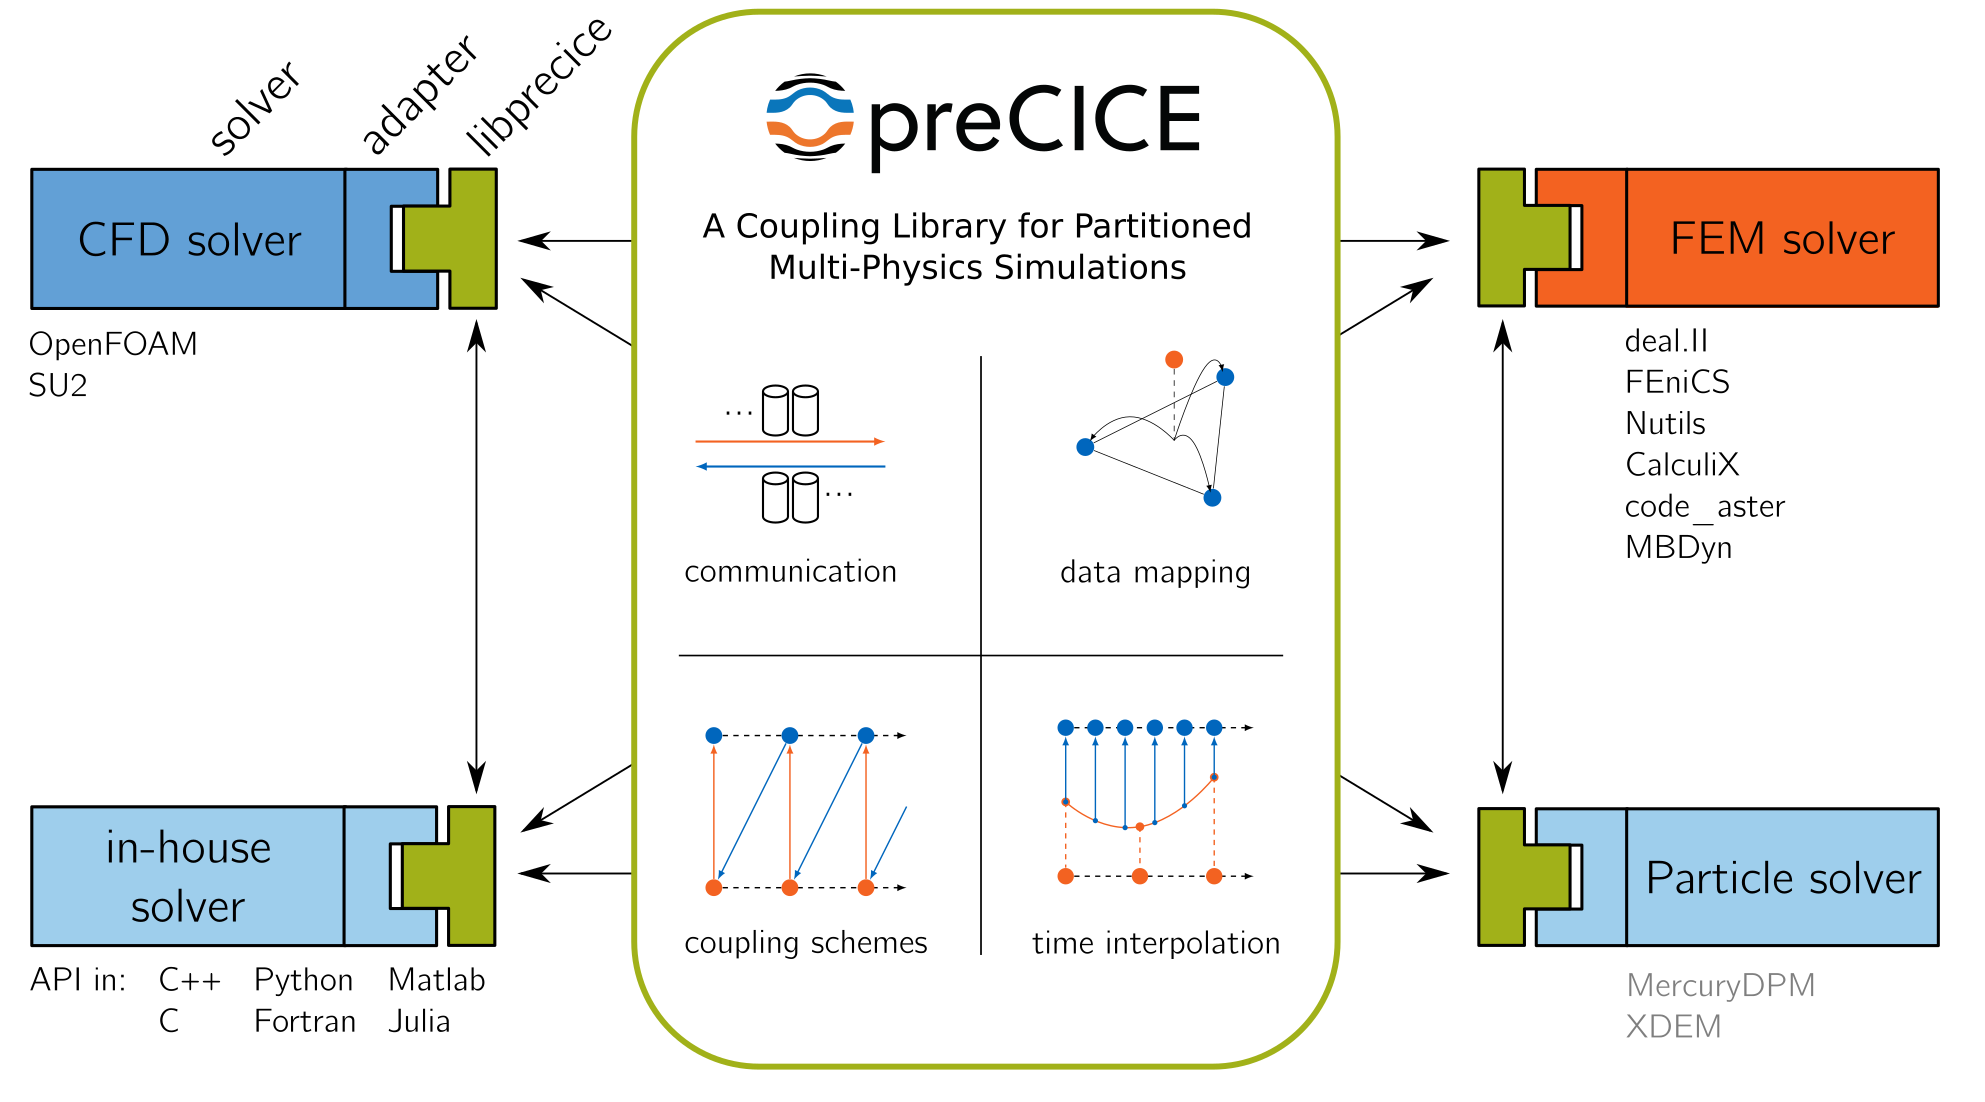
\includegraphics[width=0.9 \textwidth]{images/precice-overview.png}
	\caption{preCICE overview \cite{Chourdakis:2022}}
	\label{fig:precice:overview}
\end{figure*}


\subsubsection{OpenFOAM}

OpenFOAM\footnote{\url{https://www.openfoam.com/}}, an acronym for Open Field Operation and Manipulation, is a powerful open-source computational fluid dynamics (CFD) software package. This versatile tool provides a comprehensive suite of solvers and utilities for simulating and analyzing fluid flow, heat transfer, and related phenomena. Its open-source nature allows users to access, modify, and distribute the source code, fostering collaboration and innovation within the CFD community. Originally developed in the late 1980s, OpenFOAM has since evolved into a robust and widely-used simulation platform. It employs a finite volume method, making it particularly suitable for simulating complex fluid dynamics scenarios in various industries, including aerospace, automotive, energy, and environmental engineering.

A key strength of OpenFOAM lies in its flexibility and extensibility. Users can customize simulations by modifying the source code or by utilizing a wide range of pre-existing solvers and libraries. This adaptability makes OpenFOAM a preferred choice for researchers, engineers, and scientists seeking to tackle diverse fluid dynamics challenges. With a strong emphasis on parallel computing, OpenFOAM is capable of leveraging high-performance computing resources to accelerate simulations, enabling the analysis of large-scale and intricate fluid flow problems. Its user-friendly interface, coupled with extensive documentation and a supportive community, makes OpenFOAM an accessible tool for both beginners and experienced practitioners in the field of computational fluid dynamics.

\subsubsection{preCICE-OpenFOAM Adapter}

The preCICE-OpenFOAM adapter \cite{Chourdakis:2023} is designed to facilitate robust and efficient coupling between the preCICE library and OpenFOAM to enable multi-physics simulations. At its core, the software architecture of the adapter follows a modular design, allowing for flexibility and customization in the coupling process. The adapter consists of three distinct modules tailored for fluid flow (FF), fluid-structure interaction (FSI), and conjugate heat transfer (CHT) coupling scenarios. Each module is optimized to handle the requirements of its respective physics domain.

In the context of fluid flow coupling, the adapter incorporates modules that leverage preCICE to enable seamless communication between different fluid solvers. This modular architecture empowers users to mix and match specialized fluid dynamics solvers as needed, while preCICE maintains a standardized interface for consistent coupling. The coupling of two solvers can be performed at a shared boundary surface or on a shared volume.

For fluid-structure interaction coupling, the architecture orchestrates the interaction between OpenFOAM's fluid dynamics solvers and external structural simulation codes. This involves careful coordination to ensure accurate and efficient data exchange, enabling comprehensive simulations of scenarios involving dynamic interactions between fluids and structures.

In the realm of conjugate heat transfer coupling, the adapter's architecture facilitates the exchange of thermal information between diverse solvers within OpenFOAM and external heat transfer codes. This functionality is crucial for scenarios where temperature fields influence fluid dynamics or structural behavior, allowing for a comprehensive understanding of phenomena such as electronics cooling or combustion.

The overall design emphasizes modularity, extensibility, and adherence to established standards, making the preCICE-OpenFOAM adapter an adaptable tool for a wide range of multi-physics simulations.

\begin{comment}
\begin{itemize}
\item OpenFOAM
\begin{itemize}
\item General information
\begin{itemize}
\item Leading open-source software for computational fluid dynamics
\item Used in academia and industry
\item Scalable from laptops to supercomputers
\item Use cases: aerodynamics, aeroacoustics, particles, chemical reactions, ...
\end{itemize}
\item Setup
\begin{itemize}
\item Build upon 
\end{itemize}
\item Enables the use and modification of different solvers
\item Used mainly for CFD but also FEM simulations 
\end{itemize}
\item Adapter
\begin{itemize}
\item Enables the coupling of OpenFOAM via preCICE in different simulation scenarios
\item Exemplifies the development strategy behind preCICE: Adapter is a library for OpenFOAM and called on runtime to perform the coupling without any modification to the OpenFOAM source code
\item Different modules for different kinds of multi-physics simulations: FSI, FF, CHT
\end{itemize}
\end{itemize}	
Note:
I should introduce the OpenFOAM adapter at some point.
Lets introduce the broad concept of the adapter here and add more details, eg about the specific files that would need to be modified, later in the Challenges part
\newline
\end{comment}



\subsubsection{OpenFAST}

OpenFAST\footnote{\url{https://openfast.readthedocs.io/en/main/}} is a versatile and open-source simulation tool developed for the analysis and design of wind turbines. This software, maintained by the National Renewable Energy Laboratory (NREL) in collaboration with the wind energy community, provides a comprehensive platform for simulating the aerodynamics, structural dynamics, and turbulence effects associated with wind turbine systems.

OpenFAST is designed to meet the evolving needs of the wind energy industry, offering a modular and extensible architecture that allows users to tailor simulations to specific requirements. Its capabilities span a range of applications, including load analysis, controller design, and overall turbine performance assessment. The software incorporates advanced modeling techniques for aerodynamics, structural dynamics, and control systems, ensuring accurate representation of wind turbine behavior in various operating conditions. With a focus on high-performance computing, OpenFAST can leverage parallel processing to handle complex simulations efficiently, facilitating the analysis of large-scale wind turbine systems. The tool supports the simulation of various turbine configurations, including land-based and offshore turbines with fixed or floating platforms. This flexibility makes it a valuable tool for addressing the diverse challenges associated with wind energy projects.

On a software level, OpenFAST is a glue code for different modules which compute the various physical domains. For example, the separate module AeroDyn is used to compute the aerodynamics of a simulation case. Another module called ElastoDyn computes the structural response of the aerodynamic loads. Both tools are then coupled in runtime in the framework. OpenFAST can be interfaced with a C++ API to drive the simulation and couple the simulation to an external CFD tool.

\begin{comment}

\begin{itemize}
	\item Wind energy engineering tool developed by NREL
	\item Widely used in academia and industry
	\item Simulates the coupled aerodynamic, structural, and electrical behaviour of wind turbines as well as the control response
	\item Allows to model on- and offshore wind turbines and can be used to compute wind parks as well
	\item OpenFAST is a glue code for different modules which compute the various physical domains
	\item Takes one main input file denoted \textit{.fst} which points to more specific files for each computation module (eg AeroDyn, ServoDyn, ...)
	\item Fidelity: Does OpenFAST include computations in different fidelities? Is it a low- to mid-fidelity tool?
	\item Computes the Fluid-Structure-Interaction at blades and tower with the actuator line method
	\item Inflow field is either computed by AeroDyn or received from external CFD solver
	\item Has a dedicated C++ API for the coupling with CFD solvers
\end{itemize}

\end{comment}

%OpenFAST is a low- to mid-fidelity tool mainly used to perform turbine loads analysis and drive the detailed turbine design. The computational intensity is therefore higher than for tools used in the early design exploration phase like WISDEM, RAFT or FLORIS, but lower than highly resolved solvers necessary to understand the actual physics and check the final turbine design like ExaWind or SOWFA. 

\subsection{Software concept}

The main idea of this work is to develop a preCICE-OpenFAST adapter, a new piece of software that connects OpenFAST and preCICE. It acts as a driver code towards OpenFAST, leveraging the C++ API of the simulation program. Simultanously, it calls preCICE to communicate data and receive steering commands for the simulation. The software is configurable on runtime by two \textit{.yaml} input files. \textit{preciceInput.yaml} contains information about the coupling setup such as which variables are exchanged, which meshes are used and where the global \textit{precice-config.xml} can be found. \textit{openfastInput.yaml} adds metadata for the wind turbine simulation and points towards the OpenFAST \textit{.fst} file.\\

The software concept is presented in simplified form in Figure \ref{code:adapter}. First, the header files for important libraries are included and variables for data handling are created (lines 1-5). The script then utilizes the C++ API of OpenFAST and preCICE to instantiate and initialize both tools (lines 8-14). The \textit{FAST} object allows the access of OpenFAST while the \textit{participant} object is connected to preCICE. The coupling library controls the main time loop (line 1628) which performs the coupled simulation. First, velocity data is retrieved from the CFD solver and stored locally (line 18). The information is then passed on to OpenFAST (line 20) and updated on the internal meshes of the simulation tool. OpenFAST is called to compute the wind turbine dynamics for the next time step (line 22). The resulting blade and tower force data is extracted and stored (line 24). The updated force data is passed on to the CFD solver (line 26), after which both solvers advance in time (line 28). This loop is repeated until the simulation time is completed. Finally, preCICE and OpenFAST are destructed (lines 30-31). The software is developed and documented on GitHub\footnote{\url{https://github.com/LeonardWilleke/openfast-adapter}}. 

\begin{comment}
Main idea
\begin{itemize}
\item Write a preCICE-OpenFAST adapter (see Figure \ref{fig:setup}), a new piece of software that connects OpenFAST and preCICE
\item Acts as driver code towards OpenFAST: Calls it via the C++ API
\item Calls preCICE to communicate data and steering commands
\item Configurable by two .yaml input files
\item preciceSettings.yaml contains information about the coupling setup
\item openfastSettings.yaml contains information about the turbine simulation case
\item The concept is sketched out in Figure \ref{code:adapter}
\item line 8-10: Instantiate and initialize the interface to OpenFAST
\item line 12-14: Do the same for preCICE
\item Now both software component are ready to use
\item line 16: main time loop controlled by preCICE
\item line 18: Read velocity data from CFD solver via preCICE and store it in local variable
\item line 20: Set the velocity data in OpenFAST
\item line 22: Tell OpenFAST to compute the wind turbine dynamics for the next time step
\item line 24: Get the resulting force from OpenFAST and store it in local variable
\item line 26: Send force data to CFD solver to be used in ALM method
\item line 28: Advance both solvers in time
\item line 30-31: End the simulation after the main loop has finished
\item Developed and documented on GitHub\footnote{\url{https://github.com/LeonardWilleke/openfast-adapter}}\\
\end{itemize}
\end{comment}


\begin{comment}
	The OpenFAST adapter is something between the FMI Runner and a normal adapter:
	It executes OpenFAST like the runner but OpenFAST is a full, executable program on
	its own.
	
	\begin{figure*}[t]
	\centering
	\includegraphics[width=0.9 \textwidth]{images/precice-openfast-adapter-setup.png}
	\caption{preCICE-OpenFAST Adapter software architecture}
	\label{fig:openfast:adapter}
	\end{figure*}
\end{comment}


\begin{figure}[h!]
	\centering
	\begin{minipage}{0.9\textwidth}
		\begin{minted}{cpp}
		#include <OpenFAST.H>
		#include <precice.hpp>
		
		vector<double> readData;
		vector<double> writeData;
		
		// OpenFAST Setup
		fast::OpenFAST FAST;
		...
		FAST.init()
		// preCICE Setup
		participant = precice.participant(...);
		...
		participant.initialize();
		// main time loop
		while participant.isCouplingOngoing(): 
			// Get read data from preCICE
			participant.readData(readData, ...);
			// Set read data in OpenFAST
			FAST.setVelocity(readData, ...);
			// Compute next time step
			FAST.step();
			// Get write data from OpenFAST
			FAST.getForce(writeData, ...);
			// Send write data to preCICE
			participant.writeData(writeData, ...);
			// Advance preCICE in time
			participant.advance(dt) 
		
		participant.finalize()
		FAST.end()
		\end{minted}
	\end{minipage}
	\caption{Concept of the OpenFAST adapter: The script utilizes the C++ API to execute OpenFAST and calls preCICE to couple the simulation. For conciseness, API calls are simplified.}
	\label{code:adapter}
\end{figure}
